\section{Comparison with Other Approaches}

\citet{ingold:2008}

\citet{ingold:fischer:2014}

\citet{ingold:leifeld:2014}

Figure~\ref{fig:dvNet} highlights how we can expect high levels of sender and receiver heterogeneity. 

\begin{figure}[ht]
	\centering
	\includegraphics[width=1\textwidth]{dvNet}
	\caption{dv net}
	\label{fig:dvNet}
\end{figure}

\citet{krivitsky:handcock:2015}

% latex table generated in R 3.3.1 by xtable 1.8-2 package
% Sun Aug 21 03:32:43 2016
\begin{table}[ht]
\centering
\begingroup\normalsize
\begin{tabular}{lccccc}
   & Logit & MRQAP & LSM & ERGM & AME \\ 
  \hline
\hline
Intercept/Edges & -4.44$^{\ast}$ & -4.24$^{\ast}$ & 0.94$^{\ast}$ & -12.17$^{\ast}$ & -3.39$^{\ast}$ \\ 
   & (0.34) &  & [0.09; 1.82] & (1.40) & [-4.38; -2.50] \\ 
  \textbf{Conflicting policy preferences} &  &  &  &  &  \\ 
  $\;\;\;\;$ Business vs. NGO & -0.86 & -0.87$^{\ast}$ & -1.37$^{\ast}$ & -1.11$^{\ast}$ & -1.37$^{\ast}$ \\ 
   & (0.46) &  & [-2.42; -0.41] & (0.51) & [-2.44; -0.47] \\ 
  $\;\;\;\;$ Opposition/alliance & 1.21$^{\ast}$ & 1.14$^{\ast}$ & 0.00 & 1.22$^{\ast}$ & 1.08$^{\ast}$ \\ 
   & (0.20) &  & [-0.40; 0.39] & (0.20) & [0.72; 1.47] \\ 
  $\;\;\;\;$ Preference dissimilarity & -0.07 & -0.60 & -1.76$^{\ast}$ & -0.44 & -0.79$^{\ast}$ \\ 
   & (0.37) &  & [-2.62; -0.90] & (0.39) & [-1.55; -0.08] \\ 
  \textbf{Transaction costs} &  &  &  &  &  \\ 
  $\;\;\;\;$ Joint forum participation & 0.88$^{\ast}$ & 0.75$^{\ast}$ & 1.51$^{\ast}$ & 0.90$^{\ast}$ & 0.92$^{\ast}$ \\ 
   & (0.27) &  & [0.86; 2.17] & (0.28) & [0.40; 1.47] \\ 
  \textbf{Influence} &  &  &  &  &  \\ 
  $\;\;\;\;$ Influence attribution & 1.20$^{\ast}$ & 1.29$^{\ast}$ & 0.08 & 1.00$^{\ast}$ & 1.09$^{\ast}$ \\ 
   & (0.22) &  & [-0.40; 0.55] & (0.21) & [0.69; 1.53] \\ 
  $\;\;\;\;$ Alter's influence indegree & 0.10$^{\ast}$ & 0.11$^{\ast}$ & 0.01 & 0.21$^{\ast}$ & 0.11$^{\ast}$ \\ 
   & (0.02) &  & [-0.03; 0.04] & (0.04) & [0.07; 0.15] \\ 
  $\;\;\;\;$ Influence absolute diff. & -0.03$^{\ast}$ & -0.06$^{\ast}$ & 0.04 & -0.05$^{\ast}$ & -0.07$^{\ast}$ \\ 
   & (0.02) &  & [-0.01; 0.09] & (0.01) & [-0.11; -0.03] \\ 
  $\;\;\;\;$ Alter = Government actor & 0.63$^{\ast}$ & 0.68 & -0.46 & 1.04$^{\ast}$ & 0.55 \\ 
   & (0.25) &  & [-1.08; 0.14] & (0.34) & [-0.07; 1.15] \\ 
  \textbf{Functional requirements} &  &  &  &  &  \\ 
  $\;\;\;\;$ Ego = Environmental NGO & 0.88$^{\ast}$ & 0.99 & -0.60 & 0.79$^{\ast}$ & 0.67 \\ 
   & (0.26) &  & [-1.32; 0.09] & (0.17) & [-0.38; 1.71] \\ 
  $\;\;\;\;$ Same actor type & 0.74$^{\ast}$ & 1.12$^{\ast}$ & 1.17$^{\ast}$ & 0.99$^{\ast}$ & 1.04$^{\ast}$ \\ 
   & (0.22) &  & [0.63; 1.71] & (0.23) & [0.63; 1.50] \\ 
  \textbf{Endogenous dependencies} &  &  &  &  &  \\ 
  $\;\;\;\;$ Mutuality & 1.22$^{\ast}$ & 1.00$^{\ast}$ &  & 0.81$^{\ast}$ & 0.39 \\ 
   & (0.21) &  &  & (0.25) & [-0.12; 0.96] \\ 
  $\;\;\;\;$ Outdegree popularity &  &  &  & 0.95$^{\ast}$ &  \\ 
   &  &  &  & (0.09) &  \\ 
  $\;\;\;\;$ Twopaths &  &  &  & -0.04$^{\ast}$ &  \\ 
   &  &  &  & (0.02) &  \\ 
  $\;\;\;\;$ GWIdegree (2.0) &  &  &  & 3.42$^{\ast}$ &  \\ 
   &  &  &  & (1.47) &  \\ 
  $\;\;\;\;$ GWESP (1.0) &  &  &  & 0.58$^{\ast}$ &  \\ 
   &  &  &  & (0.16) &  \\ 
  $\;\;\;\;$ GWOdegree (0.5) &  &  &  & 8.42$^{\ast}$ &  \\ 
   &  &  &  & (2.11) &  \\ 
   \hline
\hline
\end{tabular}
\endgroup
\caption{* p $<$ 0.05. Logistic regression and ERGM results are shown with standard errors in parentheses. MRQAP provides no standard errors. LSM and AME are shown with 95\% posterior credible intervals provided in brackets.} 
\label{tab:regTable}
\end{table}


\section{Capturing Network Attributes}

To assess whether the model adequately captures the network parameters of the DV. Here we compare the observed with a set of simulated networks based on certain network statistics \citep{hunter:etal:2008}. 

See \citet{morris:etal:2008} for details on each of these parameters. 

\begin{itemize}
\item Dyad-wise shared partners - Number of dyads in the network with exactly i shared partners
\item Edge-wise shared partners - Similar to above except this counts the number of dyads with the same number of edges
\item Geodesic distances - The proportion of pairs of nodes whose shortest connecting path is of length $k$, for $k=1,2,\ldots$ Also, pairs of nodes that are not connected are classified as $k=\infty$.
\item Incoming k-star - Propensities for individuals to have connections with multiple network partners
\item Indegree - degree count is the number of nodes with the same value of the attribute as the ego node
\item Outdegree - degree count is the number of nodes with the same value of the attribute as the ego node
\end{itemize}

\begin{figure}[ht]
	\centering
	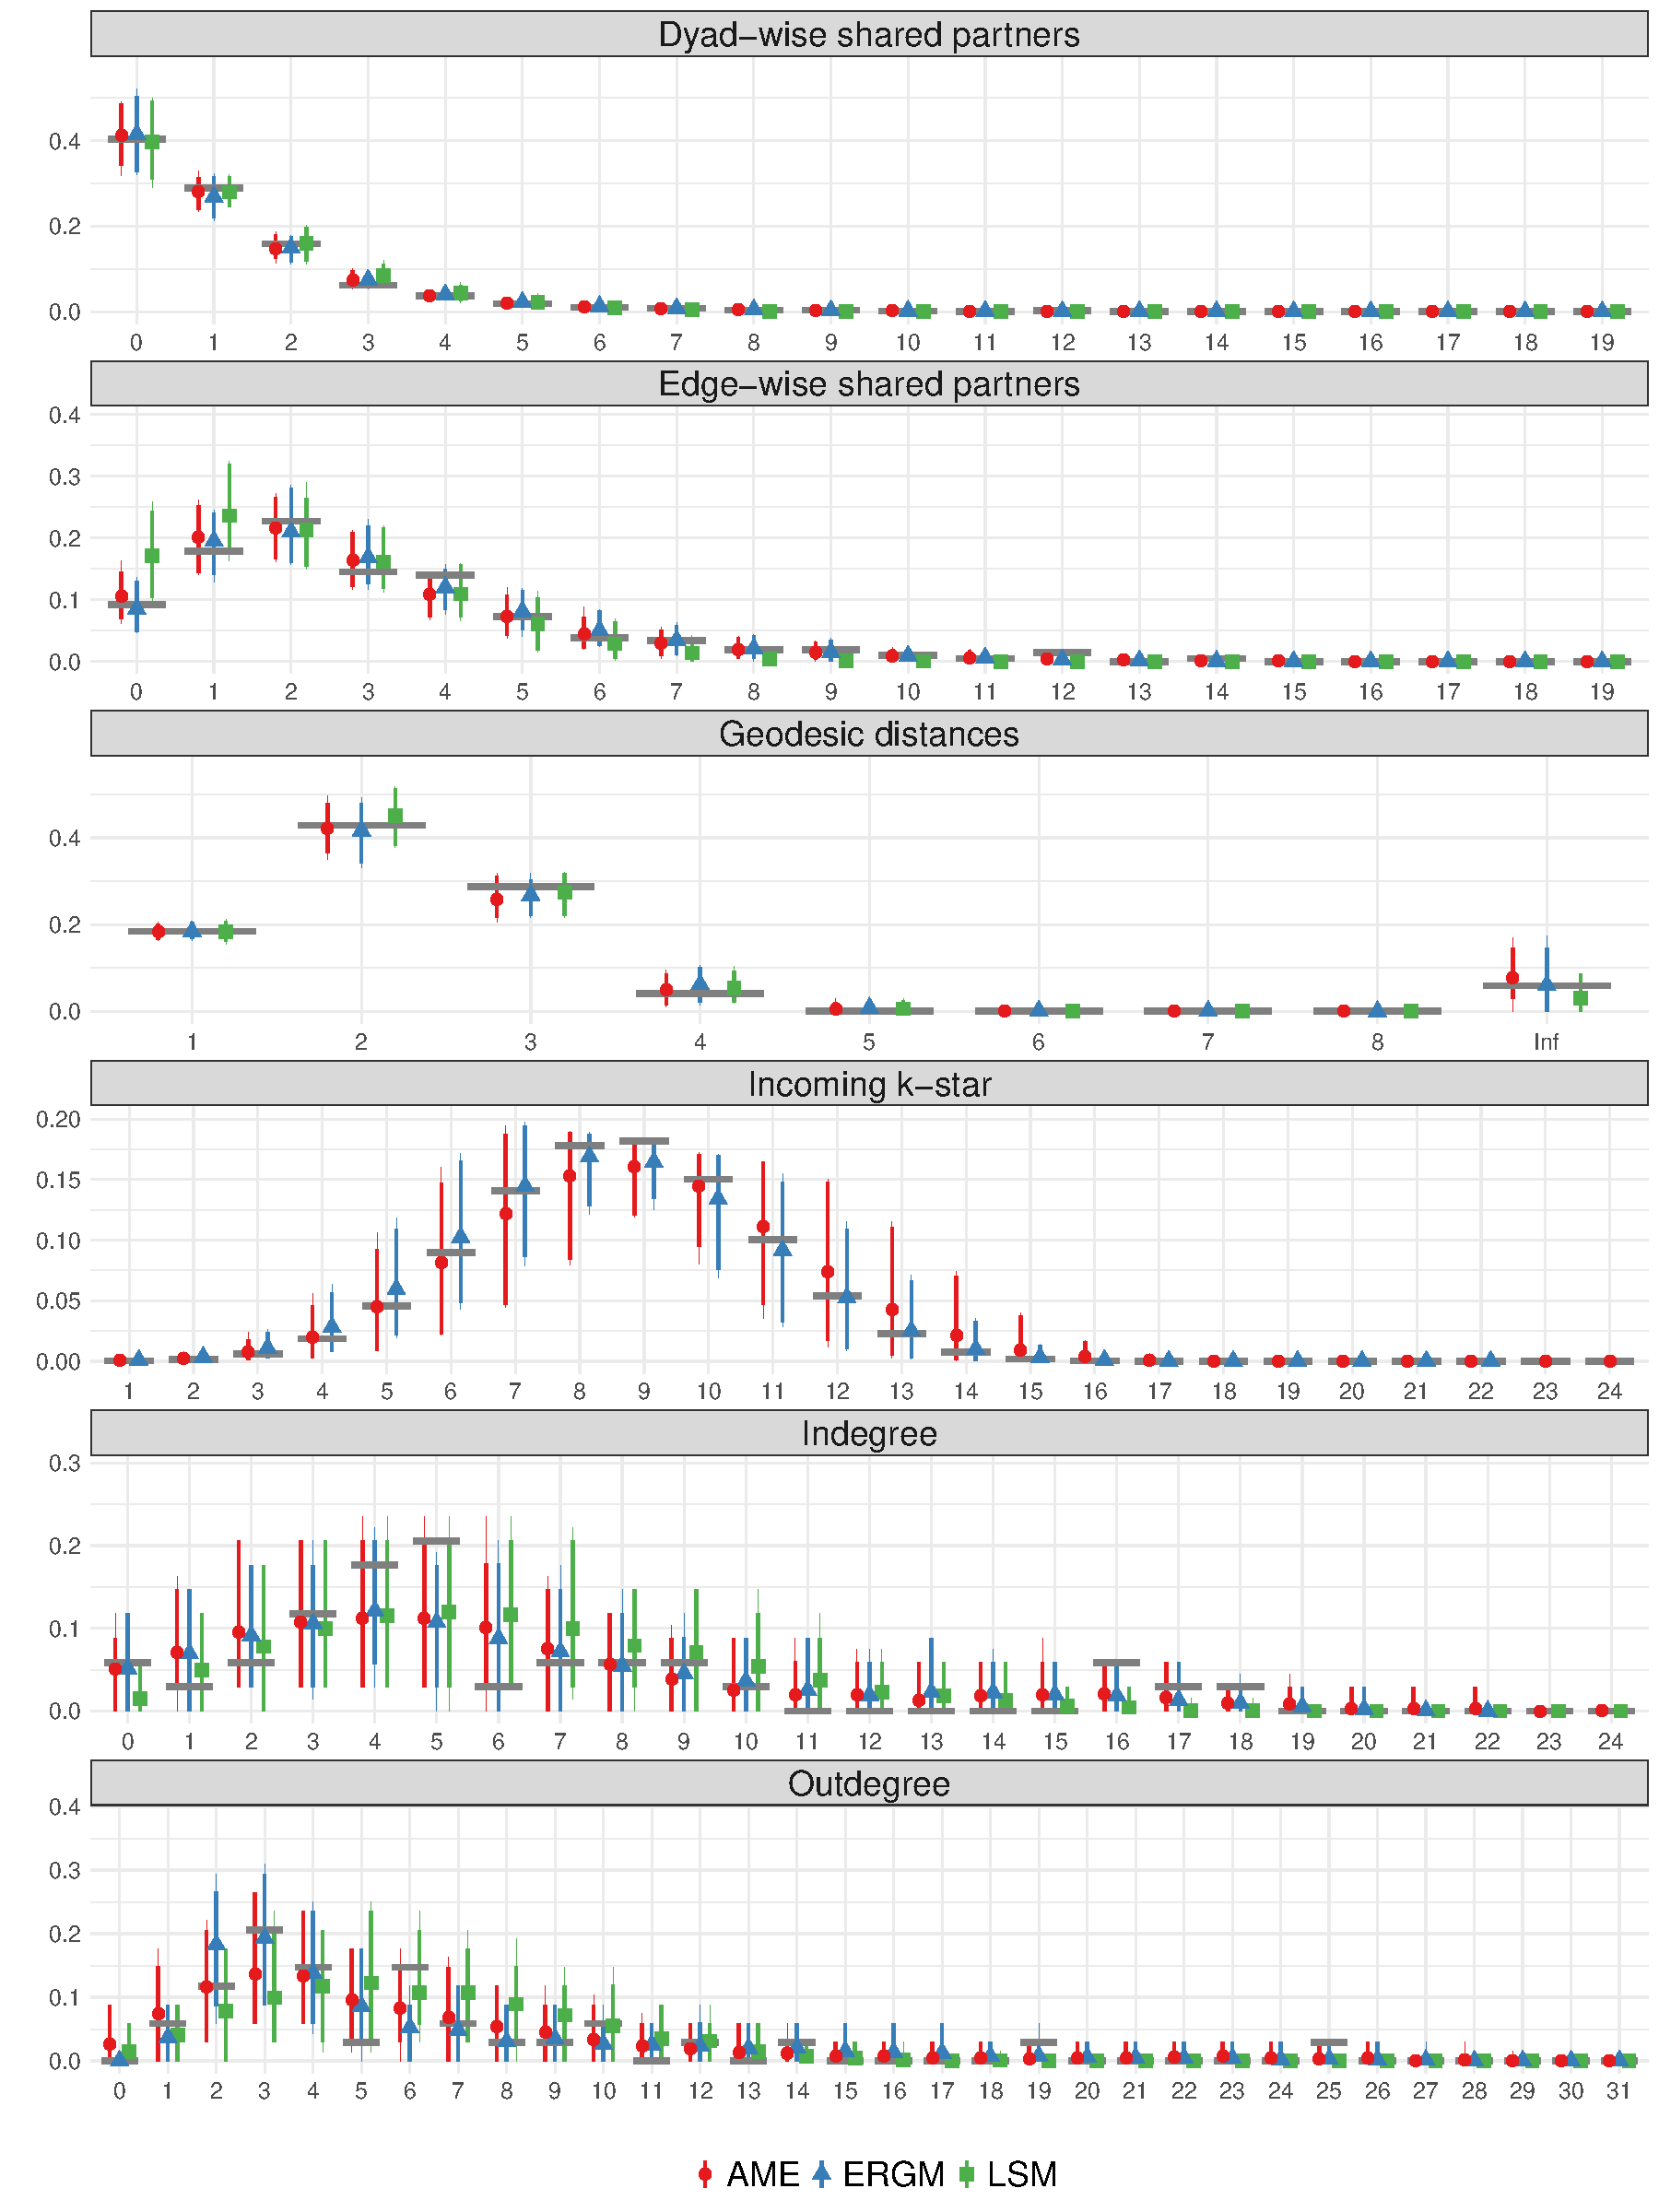
\includegraphics[width=1\textwidth]{ggGofAll}
	\caption{network stats }
	\label{fig:gofAll}
\end{figure}

Figure~\ref{fig:ergmAmePerf} give posterior predictive goodness of fit summaries for four network statistics: (1) the empirical standard deviation of the row means; (2) the empirical standard deviation of the column means; (3) the empirical within-dyad correlation; (4) a normalized measure of triadic dependence \citep{hoff:etal:2015}. 

Proportion of ties that are reciprocated. 

\begin{align}
\begin{aligned}
t(Y) &= \frac{ \sum_{i \neq j}y_{i,j} y_{j,i} }{ \sum_{i \neq j} y_{i,j} } \\
\end{aligned}
\end{align}

Number of transitive triplets

\begin{align}
\begin{aligned}
t(Y) &= \sum_{i \neq j \neq k} y_{i,j} y_{i,k} y_{j,k}
\end{aligned}
\end{align}

\begin{figure}[ht]
	\centering
	\includegraphics[width=1\textwidth]{netPerfCoef}
	\caption{Posterior predictive goodness of fit summary}
	\label{fig:ergmAmePerf}
\end{figure}

\section{Tie Formation Prediction}

\begin{figure}[ht]
	\centering
	\begin{tabular}{cc}
	\includegraphics[width=.5\textwidth]{roc} & 
	\includegraphics[width=.5\textwidth]{rocPr}	
	\end{tabular}
	\caption{ROC and separation plots}
	\label{fig:roc}
\end{figure}

% % latex table generated in R 3.3.1 by xtable 1.8-2 package
% Tue Oct 18 00:16:48 2016
\begin{table}[ht]
\centering
\begingroup\normalsize
\begin{tabular}{lcc}
  & AUC & AUC (PR) \\ 
  \hline
\hline
AME & 0.99 & 0.94 \\ 
  LSM & 0.92 & 0.68 \\ 
  ERGM & 0.91 & 0.70 \\ 
  MRQAP & 0.88 & 0.67 \\ 
  Logit & 0.88 & 0.67 \\ 
  \end{tabular}
\endgroup
\caption{Area under the curve (AUC) comparison.} 
\label{tab:aucTable}
\end{table}
